We tried both to always choose
the highest valued action, and selecting an action with probability proportional
to (rescaled) value. This method of breaking ties in the $Q$ matrix proved useful
in board game environments  where the number of states were large, but for the
other environments, it didn't add any benefit and actually caused the agent to
perform worse in some examples. The softer version of choosing proportional to
gain were less successful in all cases. A problem with sticking to the highest
value is that you tend to take one of few extreme paths: in the mines
environment you have a harder time learning to circumvent an obstacle, since
the algorithm causes you to go more in straight lines.

%Since the tie breakers, or maximisers, will not come into play for small systems more than a few times, we only use them for environments with large state-action spaces. Among the test environments, this constitutes the board game environments.

%We tested two versions of UCB policies in an attempt to shore up Sarsa($\lambda$)s unsuitability for bandit problems. The idea was to consider all states as independent bandit problems, where the UCB policies would decide the balance between exploration vs exploitation. The simpler UCB1 does not consider any upper bound on the reward and will never be satisfied, this causes it to start exploration even when faced with certain victory options. The KL-UCB considers the case where the reward is bounded. Both however, assumes long time horizons, where exploration occurs gradually. When faced with the short experiments in the competition, where the optimal approach should be to explore first, and exploit later, they fared worse than simply going for the best option. This is also due to that many of the environments have many large penalties and few rewards. Exploring anything after the first reward is found is not cost efficient. 

We chose to only use the maximiser in the two environments with large state
space; tic-tac-toe and connect four. The maximiser is triggered more often in
environments with large state spaces since ties will occur more often.
Fig~\ref{fig:tiemaximiser} shows the slight increase in cumulative reward with
maximiser enabled compared to runs without maximiser.
\begin{figure}[h]
    \centering
    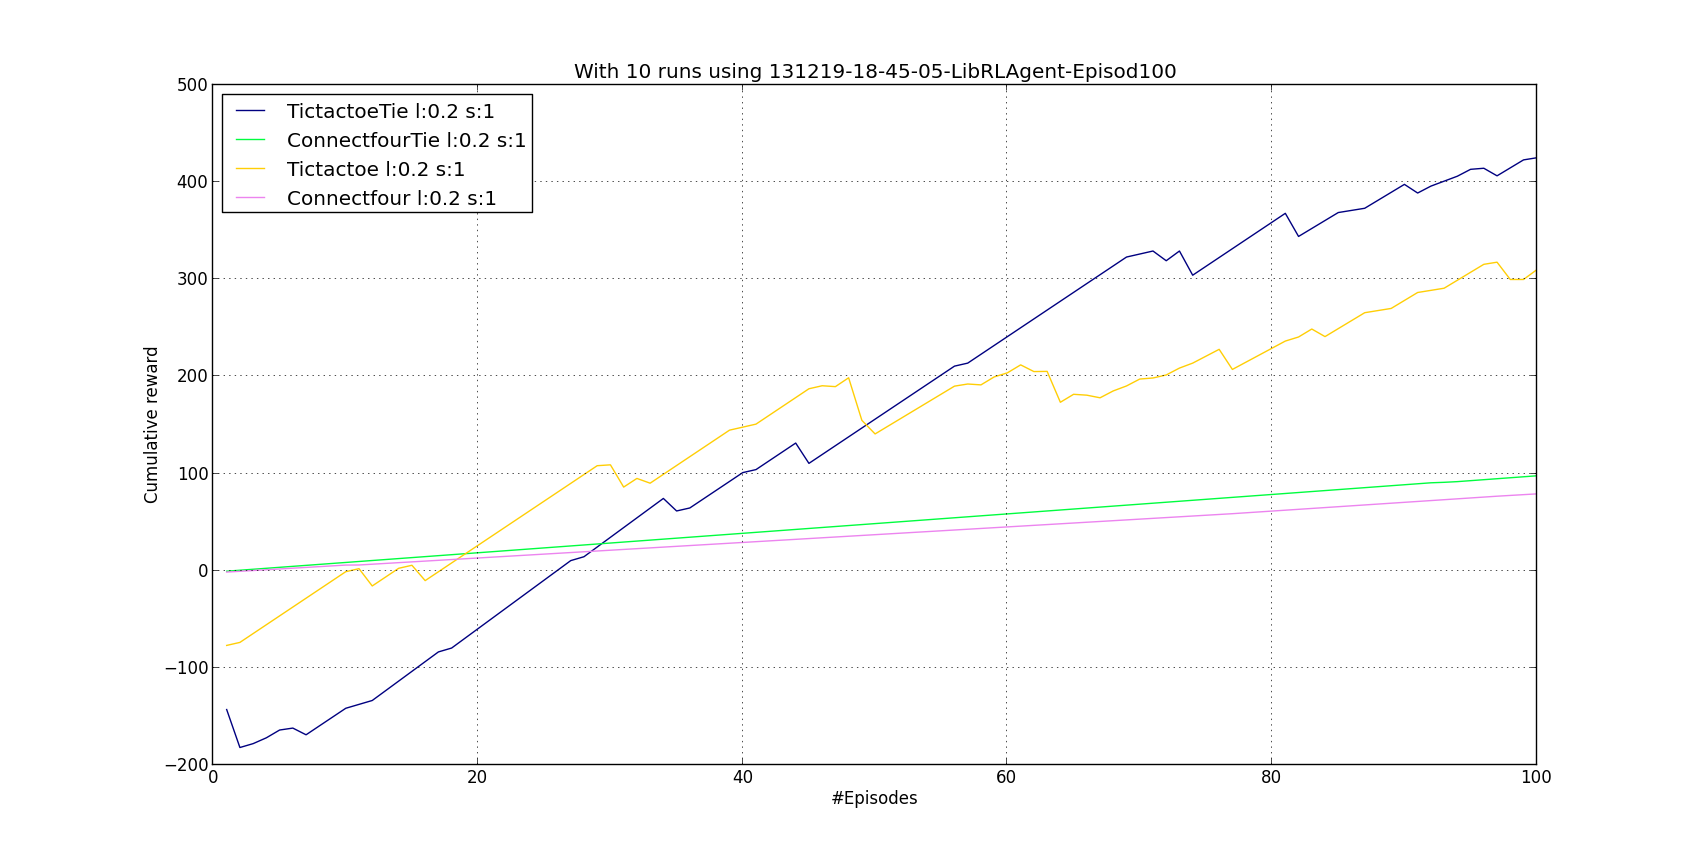
\includegraphics[width=0.5\textwidth]{../data/tiebreakerplotconnectfourtictactoe.png}
    \caption{Comparing the use of maximiser on tic-tac-toe and connect four in a experiment with 100 episodes and reward averaged over 10 runs. }
    \label{fig:tiemaximiser}
\end{figure}\\
Enabling the maximiser replaced a simple "first best" choice, which turned out
to actually be a better decision in some cases, hence we did chose to always use
the maximiser.

%When testing our agent on very different environments, from simple board games to context bandit problems. We observe that even very general approaches to improving performance against a large class of environments, might hurt the performance against other environments. We addressed large state space environments, where the state is altered gradually and good actions are good over a range of similar states, and introduced a tie breaker that tries to make informed decisions when faced with a lack of statistical data. This replaced a simple "first best" choice, which turned out to actually be a better decision in some cases. 

We tested two versions of UCB policies in an attempt to shore up
Sarsa($\lambda$)'s unsuitability for bandit problems. The idea was to consider
all states as independent bandit problems, where the UCB policies would decide
the balance between exploration vs exploitation. The simpler UCB1 does not
consider any upper bound on the reward and will never be satisfied, this causes
it to start exploration even when faced with certain victory options. The KL-UCB
considers the case where the reward is bounded. Both however, assumes long time
horizons, where exploration occurs gradually. When faced with the short
experiments in the competition, where the optimal approach should be to explore
first, and exploit later, they fared worse than simply going for the best
option. This is also due to that many of the environments have many large
penalties and few rewards. Exploring anything but the first found reward is not
cost efficient. 

The parameter space for our agent is very large, $\lambda$ decides how much we
diffuse the reward, step size $\alpha$ determines how quick the agent overwrites
old information, how we initialise the Q matrix determines if the agent is
optimistic or pessimistic when it comes to the degree of exploration. With the
UCB policies, we had the option to adjust the tendency to explore with a scalar,
we have different maximisers that attempt to exploit structure in the problems.
Naturally we didn't have time to sweep all parameters for all environments, but
we varied different parameters, keeping most constant and tried to find good
parameter values for different types of problems. At initialisation, the agent
uses known information of a problem to set the agent parameters, e.g. enables
the maximiser for large state spaces, under the assumption that the test
environments are good representations of the competition environments.

\begin{figure}[h]
    \centering
    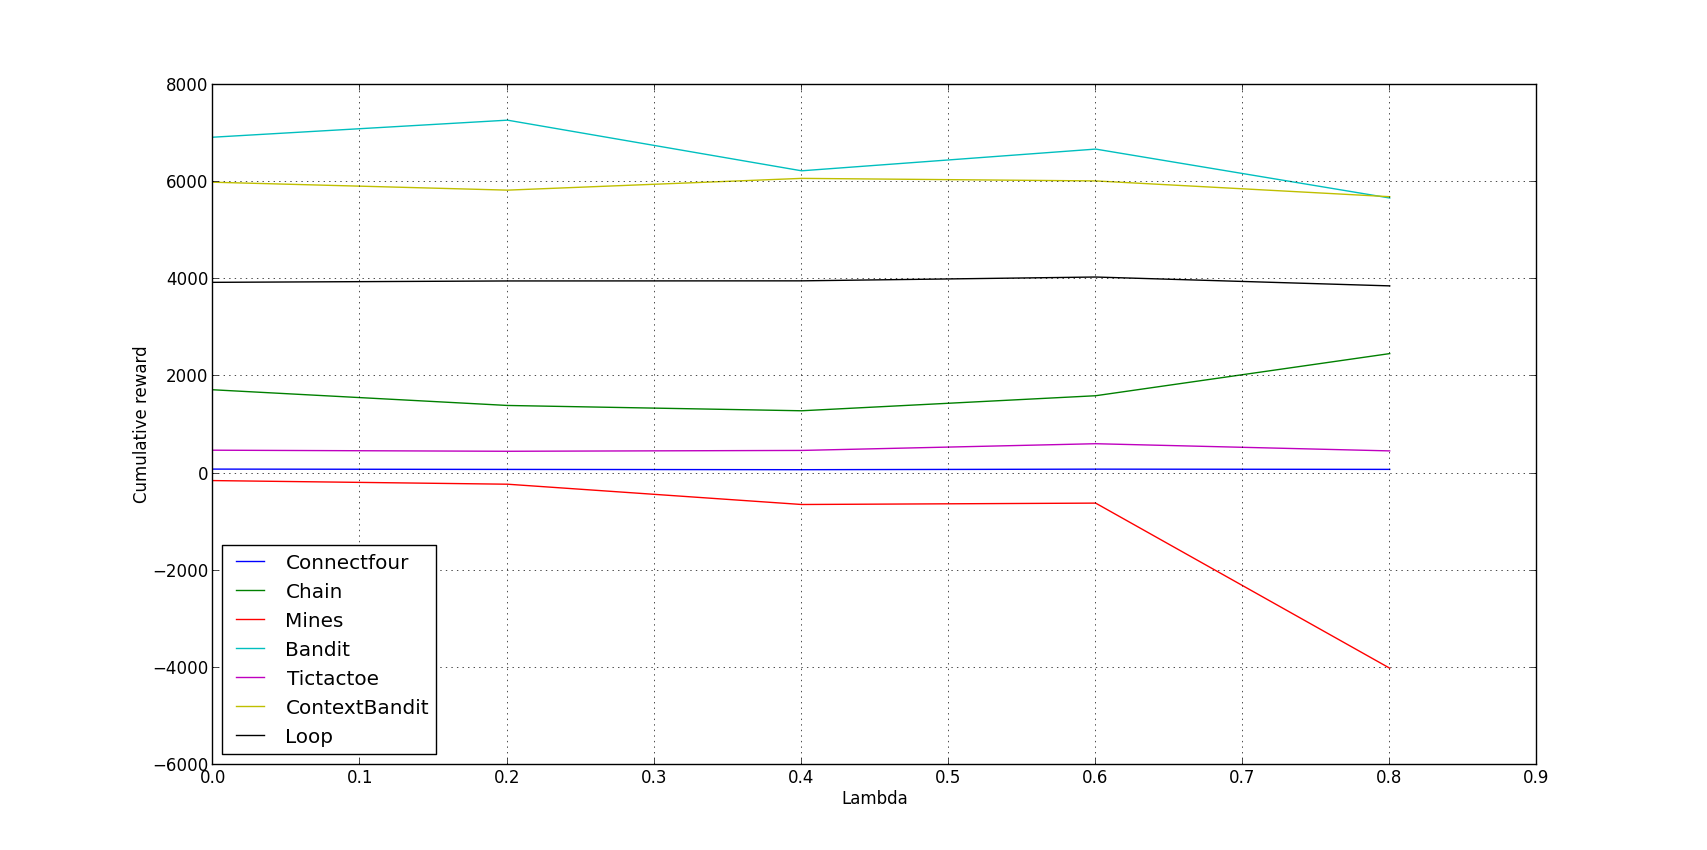
\includegraphics[width=0.5\textwidth]{../data/lambdasweepplot.png}
    \caption{How the cumulative reward changes with the different values of
        $\lambda$.}
    \label{fig:awesome_image}
\end{figure}
Figure~\ref{fig:cumreward} shows how the agents average performance over 50 runs
in a 100 episode experiment against all environments with parameters set to
$\lambda = 0.2$ and $\alpha = 1$

\begin{figure}[h!]
    \centering
    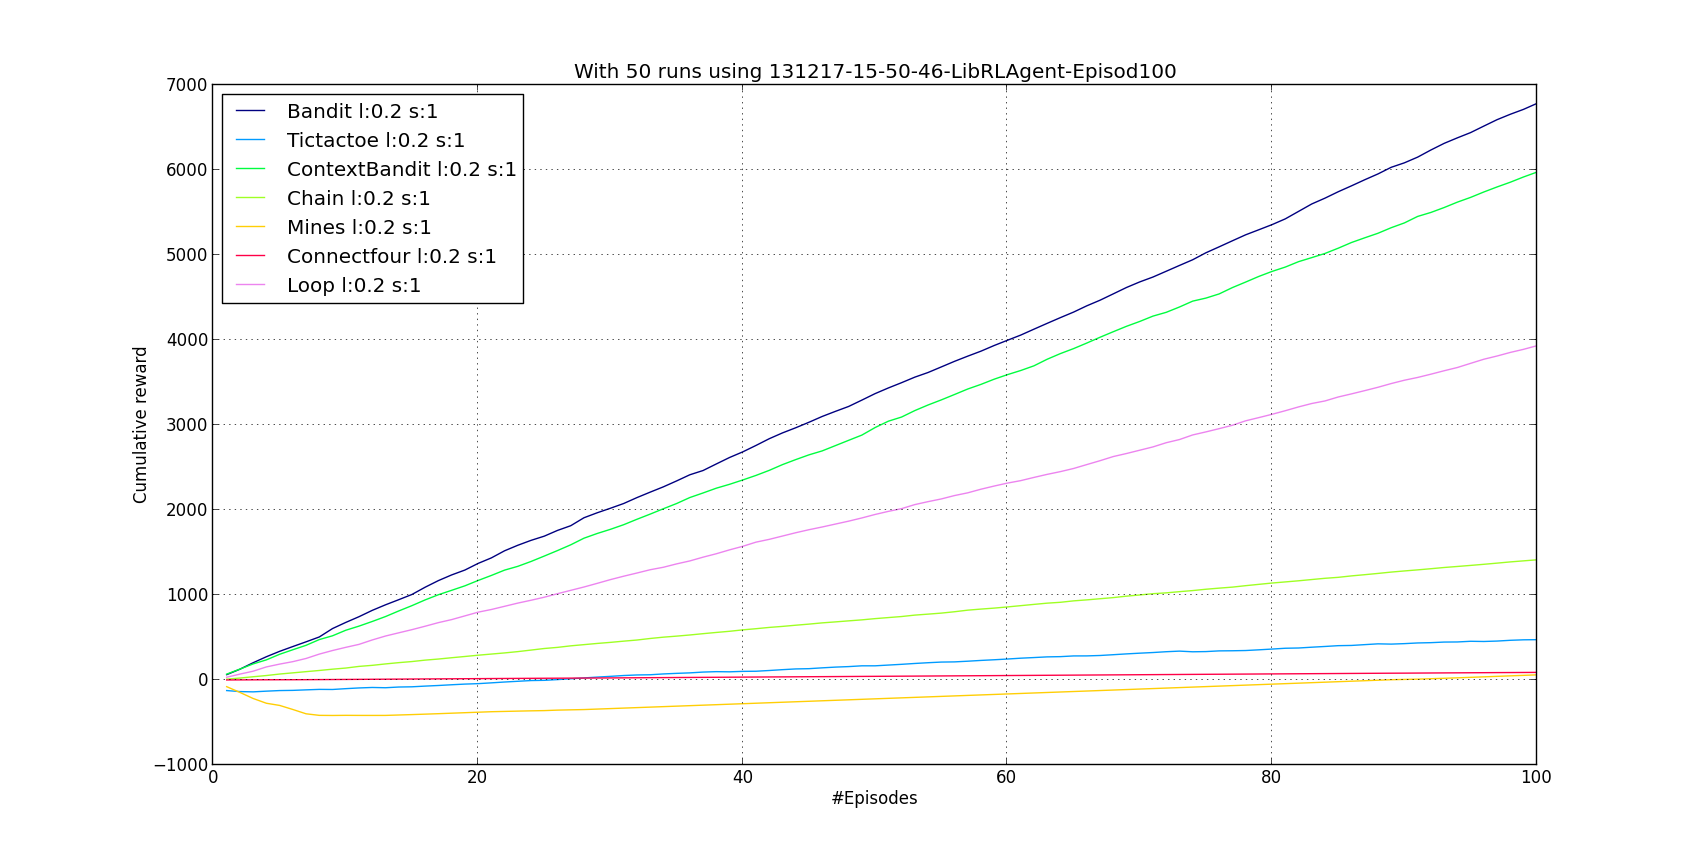
\includegraphics[width=0.5\textwidth]{../data/100episodes_50runs.png}
    \caption{Agents cumulative reward averaged over 50 runs in a experiment with
        100 episodes}
    \label{fig:cumreward}
\end{figure} 
The yellow line indicates the performance on the mines environment and the
learning phase of the agent is clear after around 10 episodes. Connect Four, red
in Fig~\ref{fig:cumreward}, has a much lower maximum reward than the other
environments hence it is closer to zero but still increasing.

Fig~\ref{fig:mineslearning} .. ``Example of how the agent learns a short path
from start to goal (yellow). The agent traverse the world 100 times, early
attempts are coloured red, later green. Hitting a mine (black) costs a penalty.
Some noise is added to the paths to make it easier to distinguish them.`` Work
on this!

\begin{figure}[h]
    \centering
    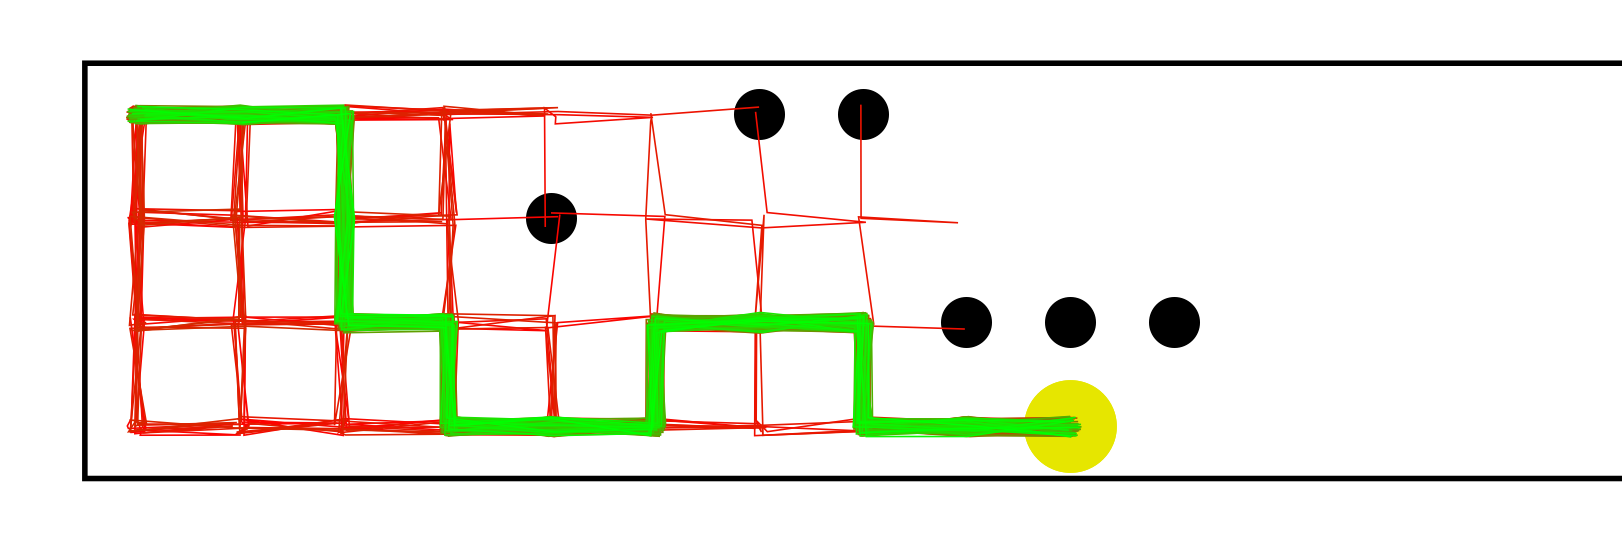
\includegraphics[width=0.5\textwidth]{../data/minPlot.png}
    \caption{Example of how the agent learns a short path from start to goal
        (yellow). The agent traverse the world 100 times, early attempts are
        coloured red, later green. Hitting a mine (black) costs a penalty. Some
        noise is added to the paths to make it easier to distinguish them.}
    \label{fig:mineslearning}
\end{figure} 

We also noticed that Sarsa($\lambda$) in its original formulation will decide on
the next action before it updates the Q matrix. In the specific case where
penalties are incurred for illegal moves, and the agents are forced to try
again, this causes the agent to perform every illegal move twice. We decided to
stick with the original, suboptimal version, since checking policy twice at each
time step is inelegant and we wanted to avoid overtraining.

We tested our agent o n

All code is publicly available via ~\cite{githubrepo}.
